\newpage
\textbf{Ejemplo 3}\\
Resolver el ejemplo 2 usando la tasa combinada.\\ \\
%\newpage %USAR SOLO SI EL SOLUCIÓN QUEDA SOLO Y ES NECESARIO BAJARLO A LA SIGUIENTE PAGINA
\textbf{Solución.}\\
%La tabla ira centrada
\begin{center}
 \renewcommand{\arraystretch}{1.5}% Margenes de las celdas
 %Creación de la cuadricula de 3 columnas
 \begin{longtable}[H]{|c|c|c|}
  %Creamos una linea horizontal
  \hline
  %Definimos el color de la primera fila
  \rowcolor[HTML]{FFB183}
  %%%%% INICIO DECLARACIÓN DE VARIABLES %%%%%%%
  %%%%%%%%%% INICIO TITULO
  \multicolumn{3}{|c|}{\cellcolor[HTML]{FFB183}\textbf{1. Asignación período focal}}                                                    \\ \hline
  \multicolumn{3}{|c|}{$pf=1\textit{ pav}$}                                                                                            \\ \hline
  %Lo que se hace aquí es mezclar las 3 columnas en una sola
  \multicolumn{3}{|c|}{\cellcolor[HTML]{FFB183}\textbf{2. Declaración de variables}}                \\ \hline
  %%%%%%%%%% FIN TITULO
  %%%%%%%%%% INICIO DE MATEMÁTICAS
  %Cada & hace referencia al paso de la siguiente columna
  \multicolumn{3}{|c|}{$j_{1} = 6\% \textit{ naav en US}$}                                         \\
  \multicolumn{3}{|c|}{$j_{2} = 20\% \textit{ naav en COL}$}                                        \\ \hline

  %%%%%%%%%% FIN DE MATEMÁTICAS
  %%%%% FIN DECLARACIÓN DE VARIABLES


  %%%%% INICIO FLUJO DE CAJA
  \rowcolor[HTML]{FFB183}
  \multicolumn{3}{|c|}{\cellcolor[HTML]{FFB183}\textbf{3. Diagrama de flujo de caja}}               \\ \hline
  %Mezclamos 3 columnas y pondremos el dibujo
  %%%%%%%%%%%%% INSERCIÓN DE LA IMAGEN
  %Deberán descargar las imágenes respectivas del drive y pegarlas en la carpeta
  %n_capitulo/img/ejemplos/1/capitulo1ejemplo1.pdf  (el /1/ es el numero del ejemplo)
  \multicolumn{3}{|c|}{ 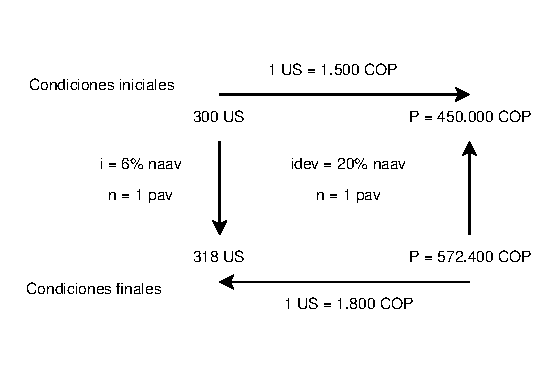
\includegraphics[trim=-78 -5 -78 -5]{3_Capitulo/img/ejemplos/3/capitulo3ejercicio3.pdf} }  \\ \hline
  %%%%%%%%%%%%% FIN INSERCIÓN DE IMAGEN
  %%%%%FIN FLUJO DE CAJA



  %%%%% INICIO DECLARACIÓN FORMULAS
  %%%%%%%%%%% INICIO TITULO
  \rowcolor[HTML]{FFB183}
  \multicolumn{3}{|c|}{\cellcolor[HTML]{FFB183}\textbf{4. Declaración de Fórmulas}}                 \\ \hline
  %%%%%%%%%%% FIN TITULO
  %%%%%%%%%%% INICIO MATEMÁTICAS

  \multicolumn{3}{|c|}{$i = i_{1}+i_{2}+i_{1}\cdot i{2}  \hspace{1cm}\textit{ Tasas combinadas}$}   \\
  \multicolumn{3}{|c|}{$j = i \cdot m \hspace{1cm}\textit{ Tasa periódica anualizada}$}             \\ \hline
  %%%%%%%%%% FIN MATEMÁTICAS
  %%%%%% INICIO DESARROLLO MATEMÁTICO
  \rowcolor[HTML]{FFB183}
  %%%%%%%%%%INICIO TITULO
  \multicolumn{3}{|c|}{\cellcolor[HTML]{FFB183}\textbf{5. Desarrollo Matemático}}                   \\ \hline
  %%%%%%%%%% FIN TITULO
  %%%%%%%%%% INICIO MATEMÁTICAS
  \multicolumn{3}{|l|}{$i_{1} = \frac{6\% \textit{ naav}}{1}= 6\% \textit{ pav}$}                   \\
  \multicolumn{3}{|l|}{$i_{2} = \frac{20\% \textit{ naav}}{1}= 20\% \textit{pav}$}                  \\
  \multicolumn{3}{|l|}{$i = 0,06+0,2+0,06 \cdot 0,2 = 0,272 \textit{ pav} \equiv i = 27,2\% \textit{ pav}$}                \\
  \multicolumn{3}{|l|}{$j = 27,2\% \cdot 1 = 27,2\% \textit{ naav}$}                                \\ \hline



  %%%%%%%%%% FIN MATEMÁTICAS
  %%%%%% FIN DESARROLLO MATEMÁTICO
  %%%%%% INICIO RESPUESTA
  \rowcolor[HTML]{FFB183}
  %%%%%%%%%%INICIO TITULO
  \multicolumn{3}{|c|}{\cellcolor[HTML]{FFB183}\textbf{6. Respuesta}}                               \\ \hline
  %%%%%%%%%% FIN TITULO
  %%%%%%%%%% INICIO RESPUESTA MATEMÁTICA
\multicolumn{3}{|c|}{$j=27,2\%\textit{ naav}$}                                                                                                \\ \hline


  %%%%%%%%%% FIN MATEMÁTICAS
  %%%%%% FIN RESPUESTA
 \end{longtable}

 %Se crean dos lineas en blanco para que no quede el siguiente texto tan pegado
 %\newline \newline %USARLO SI CREES QUE ES NECESARIO
\end{center}